\section{Intro}
\subsection{Begriffe}
\begin{concept}{Grundlegende Begriffe}\\
\begin{tikzpicture}
  % Itemized list
  \node[anchor=north west] (list) at (0, 0) {
    \begin{minipage}{\textwidth}
      \begin{itemize}
        \item $\Omega =$ Grundgesamtheit
        \item $n =$ Anzahl Objekte
        \item $X =$ Stichprobenwerte
        \item $a =$ Ausprägungen
        \item $h =$ Absolute Häufigkeit
        \item $f =$ Relative Häufigkeit
        \item $H =$ Kumulative Absolute Häufigkeit
        \item $F =$ Kumulative Relative Häufigkeit
      \end{itemize}
    \end{minipage}
  };

  % Image
  \node[anchor=north west] (image) at (4, 0) {
    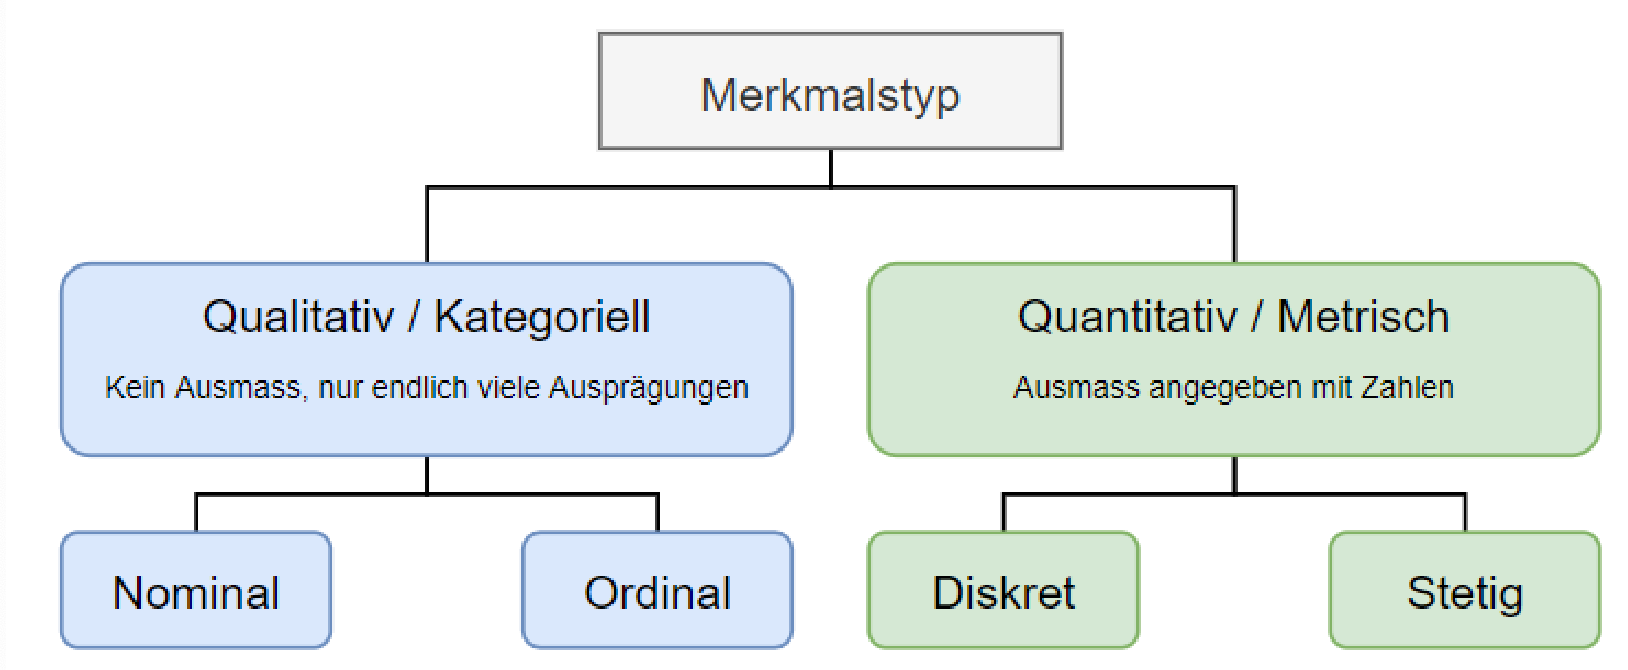
\includegraphics[width=0.5\textwidth]{images/merkmalstypen.png}
  };
\end{tikzpicture}
\end{concept}

\begin{definition}{Statistische Grundbegriffe}
\begin{itemize}
    \item \textbf{Merkmalsträger/Statistische Einheiten}: Objekte, an denen interessierende Grössen beobachtet werden
    \item \textbf{Grundgesamtheit}: Alle statistischen Einheiten, über die Aussagen gewonnen werden sollen
    \item \textbf{Vollerhebung}: Eigenschaften werden bei jedem Individuum in der Grundgesamtheit erhoben
    \item \textbf{Stichprobe}: Untersuchte Teilmenge der Grundgesamtheit (repräsentativ)
    \item \textbf{Merkmal}: Interessierende Grösse, die an den Einheiten beobachtet wird
\end{itemize}
\end{definition}

\begin{concept}{Merkmalstypen}
\begin{itemize}
    \item \textbf{Qualitativ/Kategoriell}: Ausprägung und kein Ausmass (endlich viele Ausprägungen)
    \begin{itemize}
        \item \textbf{Nominal}: Reine Kategorisierung (z.B. Parteien bei Wahlen)
        \item \textbf{Ordinal}: Ordnung vorhanden (z.B. Schulnoten)
    \end{itemize}
    \item \textbf{Quantitativ/Metrisch}: Ausmass wird mit Zahlen angegeben
    \begin{itemize}
        \item \textbf{Diskret}: Abzählbar viele Ausprägungen (z.B. Würfelwurf)
        \item \textbf{Stetig}: Alle Ausprägungen in einem reellen Intervall (z.B. Länge)
    \end{itemize}
\end{itemize}
\end{concept}

\begin{example2}{Merkmalstypen - Praktische Beispiele}
\begin{itemize}
    \item \textbf{Nominal}: Geschlecht, Automarke, Blutgruppe
    \item \textbf{Ordinal}: Bildungsabschluss, Zufriedenheit (1-5), Kaufkraft (tief/mittel/hoch)
    \item \textbf{Diskret metrisch}: Anzahl Kinder, Würfelaugen, Stockwerke
    \item \textbf{Stetig metrisch}: Temperatur, Gewicht, Länge
\end{itemize}
\end{example2}

\begin{definition}{Boxplot}\\
\begin{minipage}{0.6\columnwidth}
\begin{itemize}
  \setlength{\itemsep}{5pt}
  \item $\textcolor[HTML]{A70000}{Q_{1}},\textcolor[HTML]{005700}{ Q_{2}=x_{\text {med }}},\textcolor[HTML]{A70000}{ Q_{3}}$ (Quartile)
  \item $I Q R=Q_{3}-Q_{1}$ (Interquartilsabstand)
  \item Untere Antenne $\textcolor[HTML]{0707FF}{x_{u}}:\\ u=\min \left[Q_{1}-1.5 \cdot I Q R, Q_{1}\right]$
  \item Obere Antenne $\textcolor[HTML]{0707FF}{x_{0}}:\\ \quad o=\max \left[Q_{3}+1.5 \cdot I Q R, Q_{3}\right]$
  \item Ausreisser: $\quad x_{i}<\textcolor[HTML]{0707FF}{x_{u}} \vee x_{i}>\textcolor[HTML]{0707FF}{x_{0}}$
\end{itemize}
\end{minipage}%
\begin{minipage}{0.4\columnwidth}
  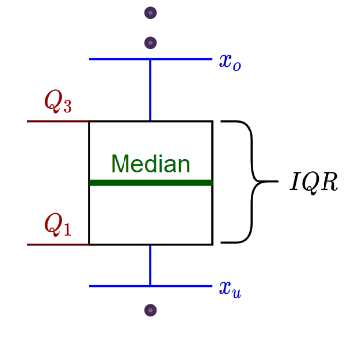
\includegraphics[width=\textwidth]{images/boxplot.png}
\end{minipage}
\end{definition}

\begin{KR}{Erstellen eines Boxplots}
\begin{enumerate}
    \item Berechne die Quartile $Q_1$, $Q_2$ (Median) und $Q_3$
    \item Bestimme den Interquartilsabstand IQR = $Q_3 - Q_1$
    \item Berechne die Grenzen für Ausreisser:
        \begin{itemize}
            \item Untere Grenze: $Q_1 - 1.5 \cdot IQR$
            \item Obere Grenze: $Q_3 + 1.5 \cdot IQR$
        \end{itemize}
    \item Zeichne Box mit:
        \begin{itemize}
            \item Unterer Rand bei $Q_1$
            \item Mittellinie bei $Q_2$
            \item Oberer Rand bei $Q_3$
        \end{itemize}
    \item Zeichne Antennen bis zum:
        \begin{itemize}
            \item Kleinsten Wert  $\geqslant$  untere Grenze
            \item Grössten Wert $\leqslant$  obere Grenze
        \end{itemize}
    \item Markiere alle Werte ausserhalb als Ausreisser
\end{enumerate}
\end{KR}

\begin{example2}{Boxplot - Praktisches Beispiel}
Gegeben sind folgende Messwerte: 2, 3, 5, 6, 7, 8, 9, 15, 50\\
\begin{enumerate}
    \item Sortiere Werte: 2, 3, 5, 6, 7, 8, 9, 15, 50
    \item Bestimme Quartile:
        \begin{itemize}
            \item $Q_1$ = 4 (25\%-Quantil)
            \item $Q_2$ = 7 (Median)
            \item $Q_3$ = 12 (75\%-Quantil)
        \end{itemize}
    \item IQR = 12 - 4 = 8
    \item Ausreisser-Grenzen:
        \begin{itemize}
            \item Untere: 4 - 1.5 · 8 = -8
            \item Obere: 12 + 1.5 · 8 = 24
        \end{itemize}
    \item 50 ist ein Ausreisser (> 24)
\end{enumerate}
\end{example2}

\subsection{Häufigkeiten}
\begin{definition}{Häufigkeiten bei nicht-klassierten Daten}
\begin{itemize}
    \item \textbf{Absolute Häufigkeit} $h_i$: Anzahl Vorkommen des Wertes $a_i$
    \item \textbf{Relative Häufigkeit} $f_i$: $f_i = \frac{h_i}{n}$
    \item \textbf{Kumulative absolute Häufigkeit} $H_i$: $H_i = \sum_{j=1}^i h_j$
    \item \textbf{Kumulative relative Häufigkeit} $F_i$: $F_i = \sum_{j=1}^i f_j = \frac{H_i}{n}$
\end{itemize}
\end{definition}

\begin{definition}{Häufigkeiten bei klassierten Daten}
Bei grossen Stichproben metrisch stetiger Merkmale werden die Werte in Klassen eingeteilt:
\begin{itemize}
    \item Klassen sind aneinandergrenzende Intervalle
    \item Obere Intervallgrenzen gehören zum nächsten Intervall
    \item Relative Häufigkeit einer Klasse = Anzahl Werte in Klasse / Stichprobengrösse
    \item Relative Häufigkeitsdichte = Relative Häufigkeit / Klassenbreite
\end{itemize}
\end{definition}

\begin{KR}{Klasseneinteilung}
\textbf{Faustregeln:}
\begin{itemize}
    \item Klassen sollten gleich breit gewählt werden
    \item Anzahl Klassen zwischen 5 und 20
    \item Anzahl Klassen sollte $\sqrt{n}$ nicht überschreiten
    \item Klassenbreite = $\frac{\text{Max - Min}}{\text{Anzahl Klassen}}$
\end{itemize}
\end{KR}

\begin{example2}{Häufigkeitsverteilung}
Noten einer Klasse: 3.5, 4.0, 4.0, 4.5, 4.5, 4.5, 5.0, 5.0, 5.5, 6.0
\begin{itemize}
    \item $n = 10$ (Stichprobengrösse)
    \item Absolute Häufigkeiten: $h_{3.5}=1$, $h_{4.0}=2$, $h_{4.5}=3$, $h_{5.0}=2$, $h_{5.5}=1$, $h_{6.0}=1$
    \item Relative Häufigkeiten: $f_{3.5}=0.1$, $f_{4.0}=0.2$, $f_{4.5}=0.3$, $f_{5.0}=0.2$, $f_{5.5}=0.1$, $f_{6.0}=0.1$
    \item Kumulative absolute Häufigkeiten: $H_{3.5}=1$, $H_{4.0}=3$, $H_{4.5}=6$, $H_{5.0}=8$, $H_{5.5}=9$, $H_{6.0}=10$
\end{itemize}
\end{example2}